\documentclass[hidelinks, 10pt,a4paper]{article}

\usepackage[english,francais]{babel}
\usepackage[utf8]{inputenc}
\usepackage{geometry}
\usepackage[T1]{fontenc}
\usepackage[pdftex]{graphicx}
\usepackage{adjustbox}
\usepackage{color}
\usepackage{setspace}
\usepackage{hyperref}
\usepackage[french]{varioref}
\usepackage{comment}
\usepackage{fancyhdr}
\pagestyle{fancy}

\renewcommand{\headrulewidth}{1pt}
\fancyhead[L]{}
\fancyhead[C]{\textbf{UML Reverse}}
\fancyhead[R]{
\includegraphics[width=2cm]{imgSTB/universite-rouen.jpg}}

%Opening
\title{\bfseries Spécification Technique des Besoins\\Projet UML Reverse}
\geometry{hmargin=2.5cm,vmargin=3cm}

\begin{document}
\maketitle
\begin{center}
\begin{tabular}{ll}
  Version~: & 0.1\\[.5em]
  Date~: & \date{\today}\\[.5em]
  Rédigé par~: & Nabil \textsc{Belkhous}\\
               & Stephen \textsc{Cauchois}\\
               & Anthony \textsc{Godin}\\
               & Yohann \textsc{Henry}\\
               & Florian \textsc{Inchingolo}\\
               & Nicolas \textsc{Meniel}\\
               & Saad \textsc{Mrabet}\\[.5em]
  Relu par~:   & Florian \textsc{Inchingolo}\\
               & Nicolas \textsc{Meniel}\\
               & Guillaume \textsc{Leroy}\\
               &\\[.5em]
  Approuvé par~: & Stéphane \textsc{Hérauville}\\[.5em]
  Signature~: &\\
\end{tabular}
\end{center}

\newpage
\begin{center}
    \section*{Mises à jour}
    \begin{tabular}{|c|c|p{8cm}|}
        \hline{\textbf{Version}} & {\textbf{Date}} & {\textbf{Modifications réalisées}}\\\hline
        {0.1} & {29/12/2015} & {Fin de la rédaction de a STB}\\\hline
        {0.1} & {11/11/2015} & {Début de la rédaction de la STB}\\\hline
    \end{tabular}
\end{center}

\newpage
%Table of contents
\tableofcontents

%Contents
\newpage
\section{Objet du projet}
Le projet \textbf{UML Reverse} vise à développer un logiciel permettant de construire des diagrammes UML graphiquement. Le projet est décomposé en deux parties~:

\subsection{Reverse}
Le programme produit un diagramme UML à partir d’un code source. Pour cette version, seul le code Java est concerné.\\
Les diagrammes créés seront sauvegardés en PlantUML et pourront être modifiés grâce au générateur de diagramme.\\
Le reverse engineering ne gérera pas les cardinalités et pourra être executé au moins en moins de 30 secondes.\\

\subsection{Générateur de diagramme}
Le générateur de diagramme permet à l’utilisateur de construire son propre diagramme UML graphiquement. \\
Il pourra soit en créer un nouveau, soit en charger un à partir d’un fichier PlantUML (avec éventuellement un fichier de paramètres propre au logiciel).\\
Le générateur permettra de modifier tous les éléments des diagrammes ainsi que leurs positions en \textit{drag and drop} (glisser-déposer).\\
L’utilisateur pourra sauvegarder ses diagrammes avec ses paramètres. ou bien les exporter.\\

\section{Documents applicables de référence}
\subsection{Expression du besoin du projet UML Reverse}
L’utilisation des diagrammes UML fait partie des outils de tout développeur informatique. Les applications (ou plugins) de bon niveau permettant d’utiliser efficacement ces diagrammes sont limités dans le domaine du libre, et ne disposent pas de toutes les fonctionnalités utiles.\\
\emph{Remarque~: Les logiciels disponibles en libre ne sont pas pérennes. En effet, souvent rachetés par des entreprises, les allers-retours entre versions libres et propriétaires sont très fréquents. Quant aux versions restées libres, elles ont pour défaut leur manque de fonctionnalités, l’ergonomie très discutable et le manque de documentation fiable.}
\subsubsection*{Objectifs}
Développer une application ergonomique permettant d’effectuer rapidement un développement informatique intégrant des diagrammes UML.
\subsubsection*{Objectifs imposés}
Afin de limiter le périmètre de l’application et d’en faire un outil exploitable, les contraintes imposées sont les suivantes~:
\begin{itemize}
\item L’application devra respecter le pseudo-langage PlantUML pour la définition des schémas. Des informations complémentaires devront être générées pour les éléments non pris en compte par PlantUML (paramètres graphiques, etc.)
\item L’application doit permettre de créer, modifier et présenter graphiquement les diagrammes dans le respect d’UML 2.
Une interface graphique doit permettre de définir les paramètres graphiques~:
\begin{itemize}
\item positionnement des éléments~;
\item sélection des éléments affichés/cachés (exemple~: dans le diagramme de classe, noms de méthodes seuls ou détails).
\end{itemize}
\item L’application doit permettre le \textit{reverse engineering}, c’est-à-dire l’extraction du diagramme de classe à partir du code source en Java d’une application. Le résultat sera stocké au format PlantUML.
\end{itemize}

\section{Lexique}
Se référer au doccument Terminologie.

\section{Fonctionnalités}
\subsection{Diagramme de cas d’utilisation}
\begin{center}
    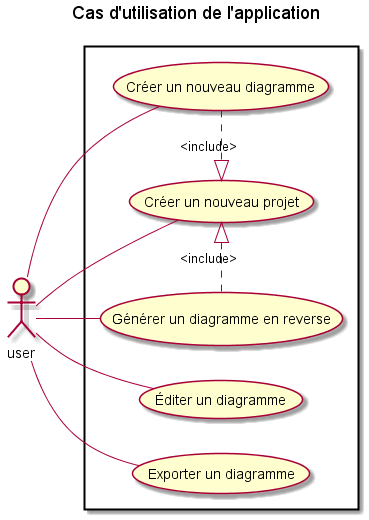
\includegraphics[width=8cm]{imgSTB/uc_general.png}
\end{center}
\newpage
\subsection{Exigences fonctionnelles de l'IHM}
\begin{center}
    \begin{tabular}{|l|p{8cm}|r|}
        \hline\multicolumn{3}{|c|}{Cas d’utilisation de l'IHM} \\\hline
        {\textbf{Identification}} & {\textbf{Description}} & {\textbf{Priorité}} \\\hline
        {IHM\_10} & {Créer un nouveau projet. (L’application crée une arboresence de dossiers pour y enregistrer par la suite des diagrammes)} & {Indispensable} \\\hline
        {IHM\_20} & {Éditer un projet} & {Indispensable} \\\hline
        {IHM\_30} & {Éditer un diagramme (suppose l’ouverture, la modification,la sauvegarde et la supression) spécifique à notre application avec ses paramètres} & {Indispensable} \\\hline
        {IHM\_40} & {Modifier le zoom du diagramme} & {Indispensable} \\\hline
        {IHM\_50} & {Charger un fichier de paramètres pour tous les diagrammes} & {Indispensable} \\\hline
        {IHM\_60} & {Expoter un fichier de paramètres qui va contenir le style} & {Indispensable} \\\hline
        {IHM\_70} & {Exporter un diagramme au format PlantUML} & {Indispensable} \\\hline
        {IHM\_80} & {Exporter un diagramme au format image/PDF} & {Optionnelle} \\\hline
        {IHM\_90} & {Imprimer un diagramme} & {Important} \\\hline
        {IHM\_100} & {Importer/charger un diagramme UML écrit en PlantUML compatible dans un projet} & {Indispensable} \\\hline
    \end{tabular}
\end{center}

\subsection{Exigences fonctionnelles des générations de diagrammes}
\begin{center}
    \begin{tabular}{|l|p{8cm}|r|}
        \hline\multicolumn{3}{|c|}{Cas d’utilisation des diagrammes} \\\hline
        {\textbf{Identification}} & {\textbf{Description}} & {\textbf{Priorité}} \\\hline
        {DIA\_10} & {Créer un nouveau diagramme de cas d’utilisation} & {Indispensable} \\\hline
        {DIA\_20} & {Créer un nouveau diagramme de classes} & {Indispensable} \\\hline
        {DIA\_30} & {Créer un nouveau diagramme de séquence} & {Optionnelle} \\\hline
        {DIA\_40} & {Créer un nouveau diagramme de paquetages} & {Optionnelle} \\\hline
        {DIA\_50} & {Créer un nouveau diagramme d’états} & {Optionnelle} \\\hline
        {DIA\_60} & {Générer un diagramme de classes par \textit{reverse engineering} sur du code Java} & {Indispensable} \\\hline
        {DIA\_70} & {Générer un diagramme de paquetages par \textit{reverse engineering} sur du code Java} & {Optionnelle} \\\hline
        {DIA\_80} & {Générer un diagramme de séquence par \textit{reverse engineering} sur du code Java} & {Optionnelle} \\\hline
    \end{tabular}
\end{center}

\newpage

\subsection{Exigences fonctionnelles des modifications possibles}
\begin{center}
    \begin{tabular}{|l|p{8cm}|r|}
        \hline\multicolumn{3}{|c|}{Cas d’utilisation des modifications possibles} \\\hline
        {\textbf{Identification}} & {\textbf{Description}} & {\textbf{Priorité}} \\\hline
        {MOD\_10} & {Ajouter un élément} & {Indispensable} \\\hline
        {MOD\_20} & {Supprimer un élément} & {Indispensable} \\\hline
        {MOD\_30} & {Afficher/cacher un élément} & {Indispensable} \\\hline
        {MOD\_40} & {Déplacer une entité} & {Indispensable} \\\hline
        {MOD\_50} & {Modifier la couleur d’une entité} & {Optionnelle} \\\hline
        {MOD\_60} & {Ajouter une flèche entre deux entités} & {Indispensable} \\\hline
        {MOD\_70} & {Modifier le style d’une flèche} & {Indispensable} \\\hline
        {MOD\_80} & {Modifier un des champs d’une flèche} & {Indispensable} \\\hline
        {MOD\_90} & {Afficher/cacher une flèche} & {Indispensable} \\\hline
        {MOD\_100} & {Supprimer une flèche} & {Indispensable} \\\hline
        {MOD\_110} & {Inverser le sens d’une flèche} & {Optionnelle} \\\hline
    \end{tabular}
\end{center}

\subsection{Précisions}
\begin{itemize}
 \item Déplacer une entité déplace tout ce qui lui est lié.
 \item Cacher/afficher une entité cache/affiche tout ce qui lui est relié.
 \item Éditer un diagramme exige qu’un projet soit déjà créé.
 \item Tous les diagrammes peuvent contenir un titre (texte). Il peut être modifié.
\end{itemize}

\newpage

\subsection{Modification d’un diagramme de cas d’utilisation}
\subsubsection{Schema fonctionnel d’utilisation}
\begin{center}
    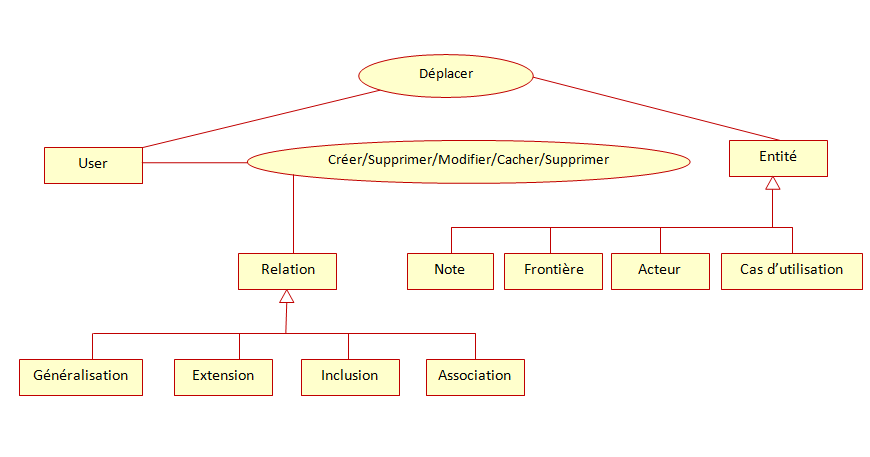
\includegraphics[width=14cm]{imgSTB/E-R-UseCase.png}
\end{center}
\subsubsection{Précisions}
\begin{itemize}
 \item Une note contient un texte quelconque.
 \item Une frontière contient un nom.
 \item Un acteur contient un nom. 
 \item Un cas d’utilisation contient un texte. Ce texte peut contenir des séparations en trait continu, en pointillés ou en double trait continu.
 \item Une relation est une flèche.
\end{itemize}

\subsubsection{Liste des cas d’utilisation supplémentaires}
\begin{center}
    \begin{tabular}{|l|p{8cm}|r|}
        \hline\multicolumn{3}{|c|}{Modification d’un diagramme de cas d’utilisation} \\\hline
        {\textbf{Numéro}} & {\textbf{Description}} & {\textbf{Priorité}}\\\hline
        {USE\_10} & {Modifier le texte d’une note} & {Indispensable} \\\hline
        {USE\_20} & {Modifier le nom d’une frontière. Ce nom est une chaîne de caractères quelconque.} & {Indispensable} \\\hline
        {USE\_30} & {Modifier le nom d’un acteur. Ce nom est une chaîne de caractères quelconque.} & {Indispensable} \\\hline
        {USE\_40} & {Modifier le texte d’un cas d’utilisation. Ce texte est une chaîne de caractères quelconque.} & {Indispensable} \\\hline
    \end{tabular}
\end{center}

\subsection{Modification d’un diagramme de classes}
  \subsubsection{Schéma fonctionnel d’utilisation}
    \begin{center}
	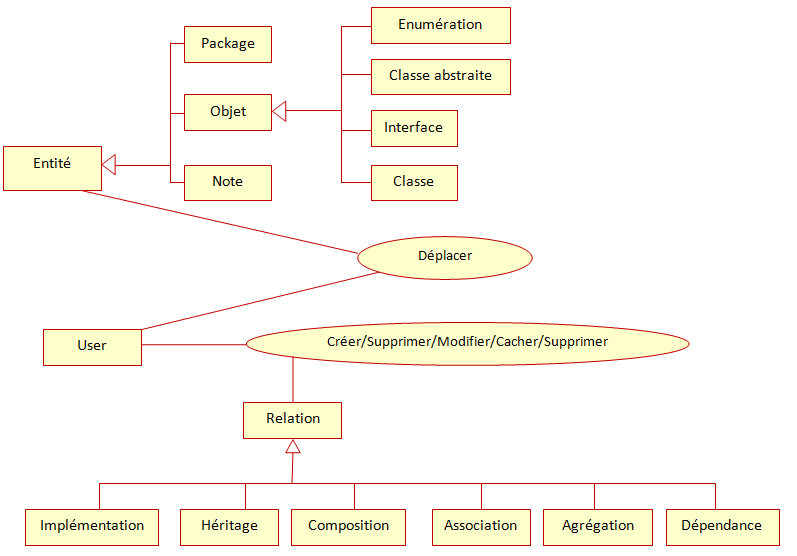
\includegraphics[width=14cm]{imgSTB/E-R-Class.png}
    \end{center}

\subsubsection{Précisions}
\begin{itemize}
 \item Les objets contiennent tous les éléments suivants~:
 \begin{itemize}
    \item au moins un nom~: un mot seulement~;
    \item au moins un type~: classe, interface, etc.~; 
    \item éventuellement des attributs~: un texte quelconque sans parenthèse ouvrante ni fermante~;
    \item éventuellement des méthodes~: un texte quelconque contenant au moins une parenthèse ouvrante ou fermante.
\end{itemize}
 \item Un attribut et une méthode peuvent avoir une (et une seule) visibilité éditable~: publique, privée, protégée ou \textit{package-private}.
 \item Une note contient un texte.
 \item Une relation est une flèche.
 \item Un paquetage contient un nom et éventuellement des objets qui ne sont pas considérés comme des entités mais comme des éléments.
\end{itemize}

\newpage

\subsubsection{Liste des cas d’utilisation supplémentaires}
\begin{center}
    \begin{tabular}{|l|p{8cm}|r|}
        \hline\multicolumn{3}{|c|}{Modification d’un diagramme de classes} \\\hline
        {\textbf{Identification}} & {\textbf{Description}} & {\textbf{Priorité}} \\\hline
        {CLA\_10} & {Modifier le nom d’un objet} & {Indispensable} \\\hline
        {CLA\_20} & {Changer le type d’un objet} & {Indispensable} \\\hline
        {CLA\_30} & {Modifier un attribut} & {Indispensable} \\\hline
        {CLA\_40} & {Modifier une méthode} & {Indispensable} \\\hline
        {CLA\_50} & {Modifier la visibilité d’un attribut ou d’une méthode} & {Indispensable} \\\hline
        {CLA\_60} & {Modifier le texte d’une note} & {Indispensable} \\\hline
        {CLA\_70} & {Modifier le nom d’un paquetage} & {Indispensable} \\\hline
        {CLA\_80} & {Modifier un objet (son nom, ses attributs et ses méthodes) contenu par un paquetage} & {Indispensable} \\\hline
        {CLA\_90} & {Redimensionner un paquetage et un objet} & {Indispensable} \\\hline
    \end{tabular}
\end{center}


\subsection{Cas d’utilisation de modification d’un diagramme de séquence}
\subsubsection{Schéma fonctionnel d’utilisation}
\begin{center}
    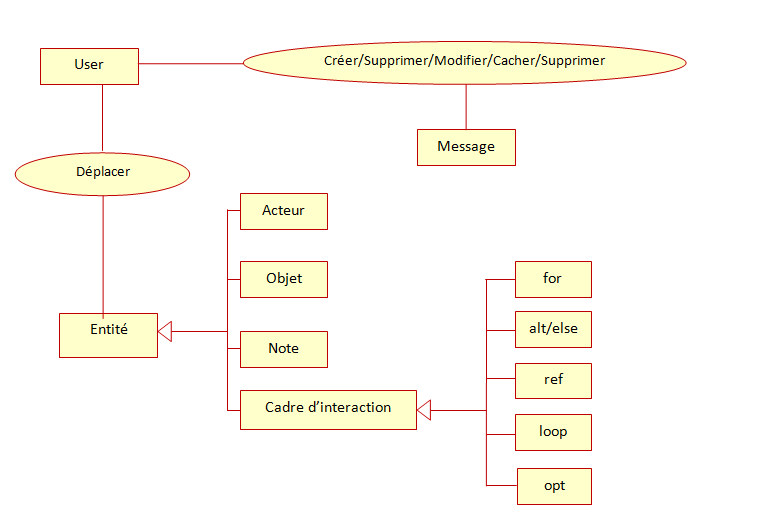
\includegraphics[width=14cm]{imgSTB/E-R-Sequence.png}
\end{center}

\subsubsection{Précisions}
\begin{itemize}
 \item Un acteur contient un nom.
 \item Un objet contient un nom (un unique mot) et d’une ligne de «~temps de vie~».
 \item Une note contient un texte.
 \item Une relation est une flèche.
 \item Un cadre d’itération contient un texte et regroupe des messages.
 \item Un cadre else suit imédiatement un cadre alt. Sans alt, il ne peut y avoir de else.
 \item Un message est une flèche.
 \item Déplacer un objet déplace aussi tout ce qui lui est lié, c’est-à-dire les flèches, les cadres d’itération et sa ligne de vie.
\end{itemize}

\subsubsection{Liste des cas d’utilisation supplémentaires}
\subsubsection{Liste des cas d’utilisation}
\begin{center}
    \begin{tabular}{|l|p{8cm}|r|}
        \hline\multicolumn{3}{|c|}{Modification d’un diagramme de séquence} \\\hline
        {\textbf{Numéro}} & {\textbf{Description}} & {\textbf{Priorité}}\\\hline
        {SEQ\_10} & {Modifier le nom d’un acteur. Ce nom est une chaîne de caractères quelconque} & {Indispensable}\\\hline
        {SEQ\_20} & {Modifier le nom d’un objet} & {Indispensable}\\\hline
        {SEQ\_30} & {Modifier le texte d’une note} & {Indispensable}\\\hline
        {SEQ\_40} & {Modifier le type d’un cadre d’itération~: for, alt, ref, etc.} & {Indispensable}\\\hline
        {SEQ\_50} & {Modifier le texte contenu dans un cadre d’itération} & {Indispensable}\\\hline
        {SEQ\_60} & {Modifier les messages contenus dans un cadre d’itération} & {Indispensable}\\\hline
	{SEQ\_70} & {Modifier la ligne de temps d’un objet} & {Indispensable}\\\hline
    \end{tabular}
\end{center}


\section{Exigences fonctionnelles}
\begin{center}
    \begin{tabular}{|l|p{10cm}|}
        \hline{\textbf{Identifiant}} & {\textbf{Description}}\\\hline
        {EXF\_10} & {L’application est codée en Java.}\\\hline
        {EXF\_20} & {L’interface graphique doit être fonctionnelle, pratique et adaptée aux besoins.}\\\hline
        {EXF\_30} & {Le \textit{reverse} permet de générer un diagramme à partir d'un fichier compatible Java 7.}\\\hline
        {EXF\_40} & {L’application implémente tous les élements d’un diagramme UML2 pour les diagrammes compatibles.}\\\hline
        {EXF\_50} & {À tout moment de l’édition d’un diagramme non vide, un fichier PlantUML compilable peut être généré à partir du diagramme.}\\\hline
        {EXF\_60} & {L’utilisateur ne peut pas avoir deux entités du même nom dans un diagramme.}\\\hline
        {EXF\_70} & {Le code de l’application doit être modulaire.}\\\hline
        {EXF\_80} & {L’application doit fonctionner sur les ordinateurs de l’Université.}\\\hline
    \end{tabular}
\end{center}

\section{Exigences}
  \subsection{Exigences fonctionnelles}
    \begin{center}
	\begin{tabular}{|l|p{10cm}|}
	    \hline{\textbf{Identifiant}} & {\textbf{Description}}\\\hline
	    {EXF\_20} & {L’interface graphique doit être fonctionnelle, pratique et adaptée aux besoins.}\\\hline
	    {EXF\_30} & {Le \textit{reverse} permet de générer un diagramme à partir d'un fichier compatible Java 7.}\\\hline
	    {EXF\_40} & {L’application implémente tous les élements d’un diagramme UML2 pour les diagrammes compatibles.}\\\hline
	    {EXF\_50} & {À tout moment de l’édition d’un diagramme non vide, un fichier PlantUML compilable peut être généré à partir du diagramme.}\\\hline
	    {EXF\_60} & {L’utilisateur ne peut pas avoir deux entités du même nom dans un diagramme.}\\\hline
	\end{tabular}
    \end{center}
  \subsection{Exigences de qualités}
    \begin{center}
      \begin{tabular}{|l|p{10cm}|}
	\hline{\textbf{Identifiant}} & {\textbf{Description}}\\\hline
	{EXF\_70} & {Le code de l’application doit être modulaire.}\\\hline
      \end{tabular}
    \end{center}
  \subsection{Exigences techniques}
    \begin{center}
      \begin{tabular}{|l|p{10cm}|}
	\hline{\textbf{Identifiant}} & {\textbf{Description}}\\\hline
	{EXF\_10} & {L’application est codée en Java.}\\\hline
	{EXF\_80} & {L’application doit fonctionner sur les ordinateurs de l’Université.}\\\hline
      \end{tabular}
    \end{center}
\end{document}